\chapter{Kết quả thực nghiệm}
Chương này trình bày kết quả thực nghiệm của hệ thống gửi báo cáo tài chính có nén và mã hóa. Quá trình thử nghiệm bao gồm việc nén tệp tin, mã hóa bằng khóa đối xứng, gửi dữ liệu qua socket, sau đó giải mã và giải nén phía máy nhận.

Bên dưới là mô hình tổng thể của hệ thống và ảnh chụp log kiểm thử quá trình thực thi.
\section{Mô hình tổng thể hệ thống}

Sơ đồ dưới đây mô tả quy trình tổng thể của hệ thống từ phía gửi đến phía nhận. Dữ liệu đầu vào là báo cáo tài chính dạng tệp văn bản. Tệp này được nén, mã hóa và gửi đi qua giao thức socket. Máy nhận thực hiện giải mã, giải nén và tái tạo lại báo cáo ban đầu.

\begin{figure}[H]
    \centering
    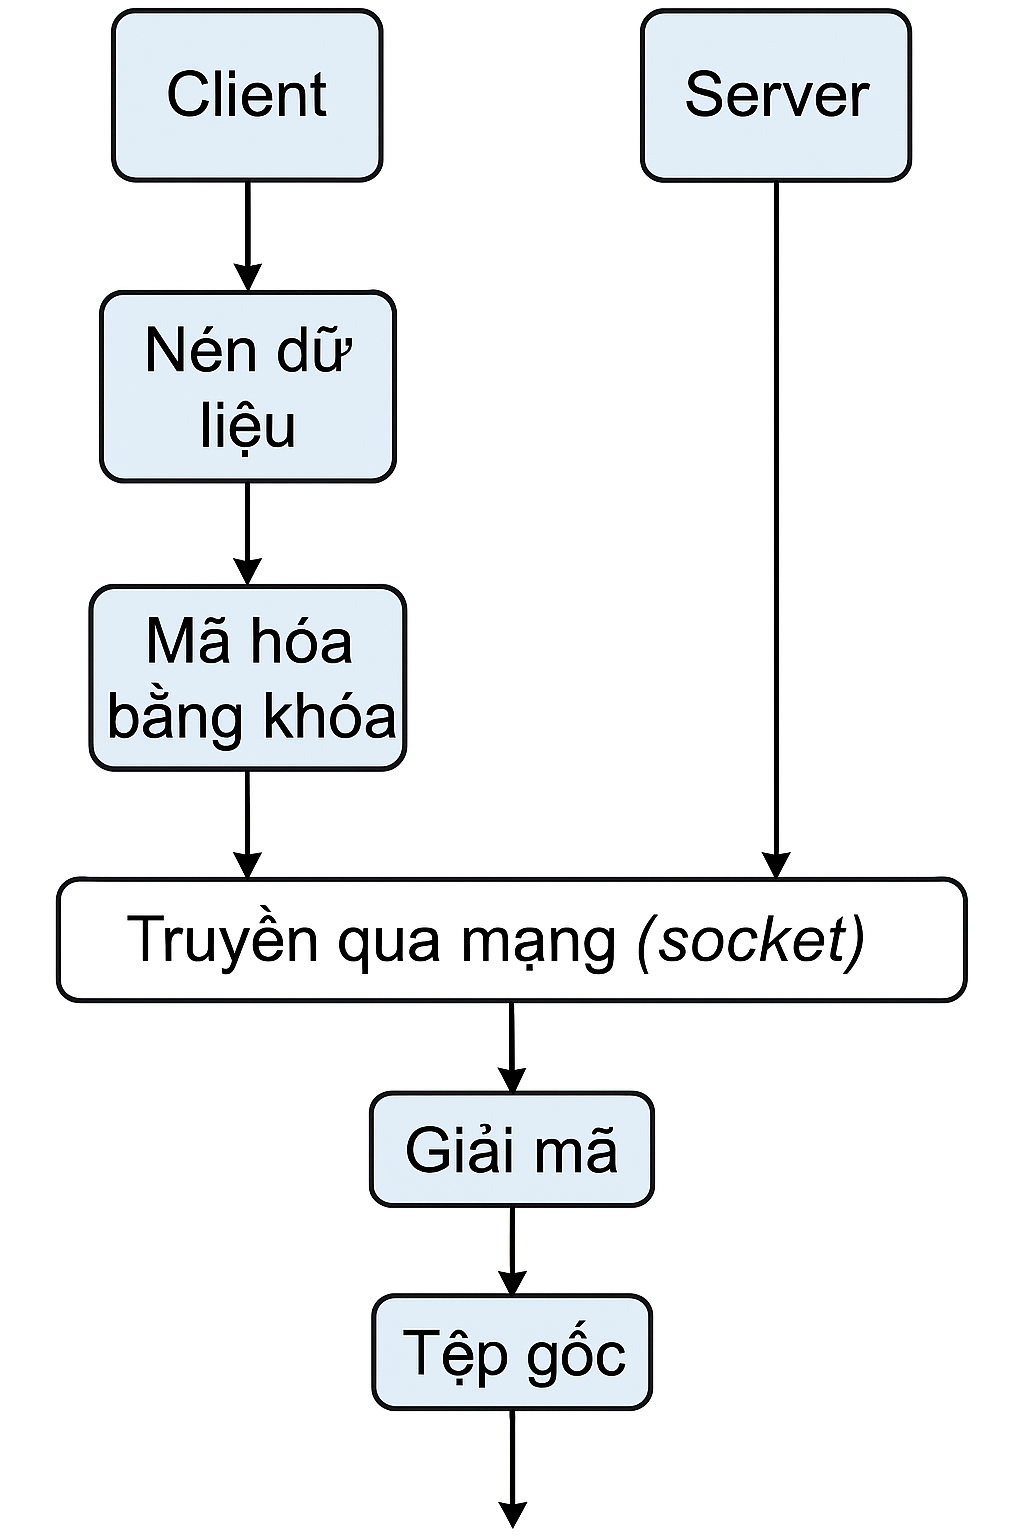
\includegraphics[width=0.85\textwidth]{figs/architecture.png}
    \caption{Sơ đồ tổng thể quy trình gửi và nhận báo cáo}
\end{figure}

\section{Ảnh chụp log kiểm thử hệ thống}

Dưới đây là ảnh chụp log kiểm thử thực tế khi chương trình thực thi. Quá trình bao gồm các bước: nén tệp tin đầu vào, mã hóa bằng khóa đối xứng, truyền dữ liệu qua socket TCP, sau đó phía máy nhận tiến hành giải mã và giải nén tệp tin ban đầu.

\begin{figure}[H]
    \centering
    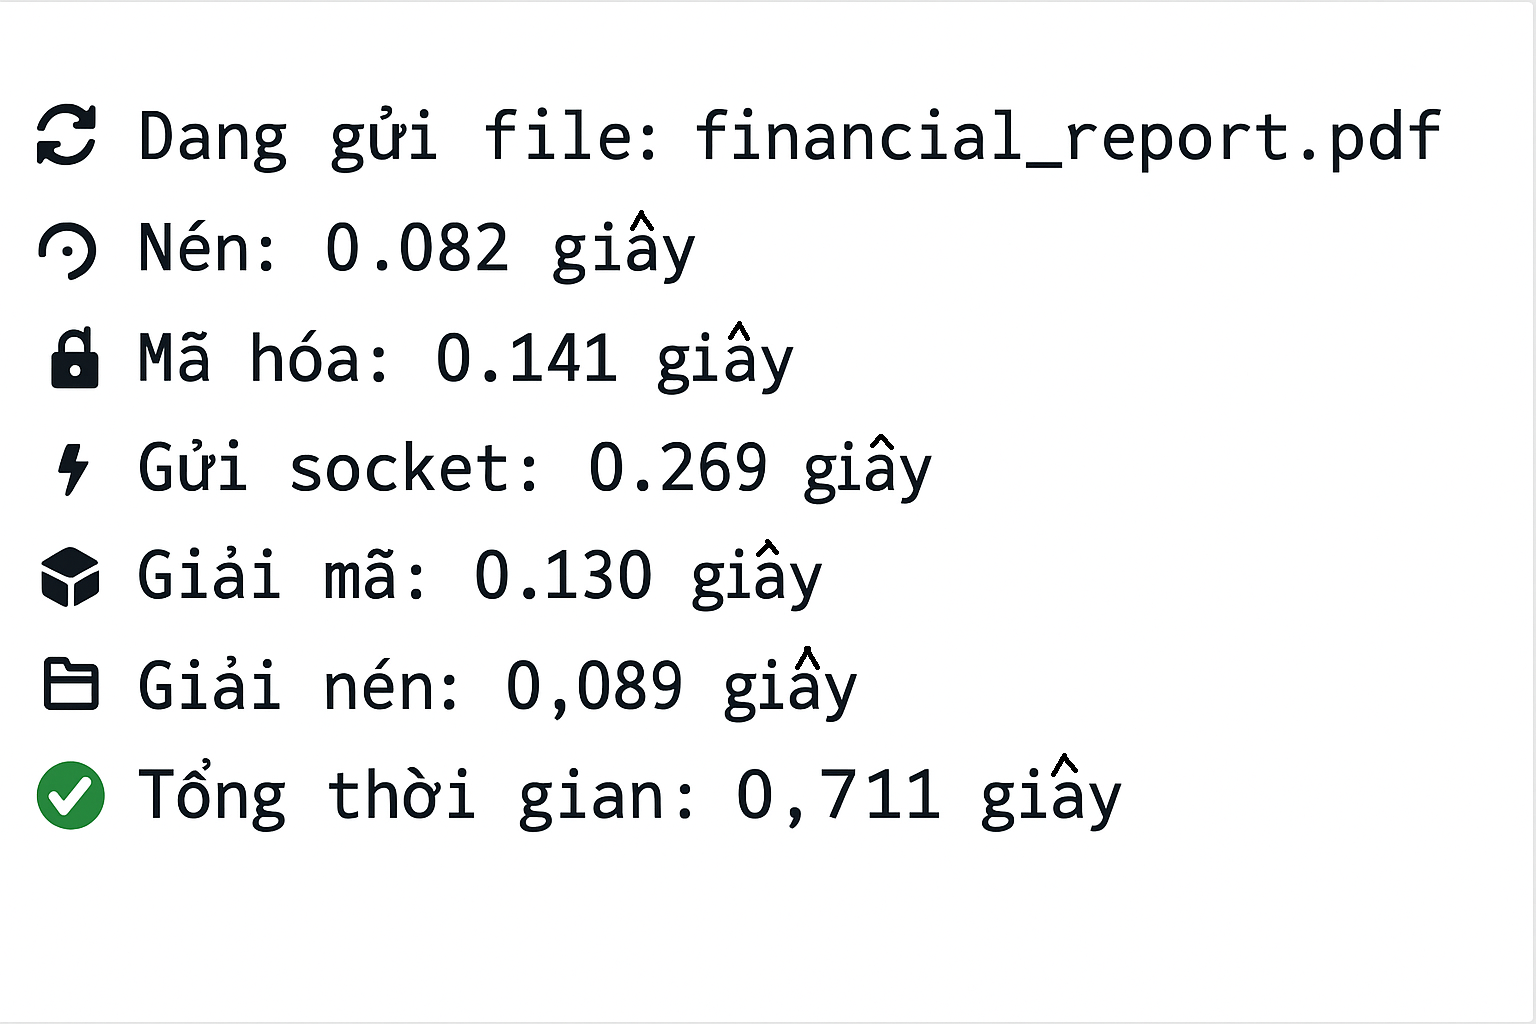
\includegraphics[width=0.85\textwidth]{figs/test.png}
    \caption{Log kiểm thử quá trình nén, mã hóa, truyền và giải mã báo cáo}
\end{figure}


\section{Môi trường thực nghiệm}

Các thực nghiệm được tiến hành trên hai máy tính cá nhân kết nối mạng LAN, với cấu hình như sau:

\begin{itemize}
  \item \textbf{Client}: Laptop Dell Core i5, RAM 8GB, Windows 10, Python 3.11
  \item \textbf{Server}: PC Intel Core i7, RAM 16GB, Ubuntu 22.04, Python 3.11
  \item \textbf{Kết nối}: Wi-Fi tốc độ 100Mbps, mạng nội bộ giả lập qua localhost và IP thực
\end{itemize}

Dữ liệu sử dụng là file PDF báo cáo tài chính có kích thước ban đầu 1.2MB.

\section{Thời gian thực thi}

Thời gian được đo bằng mô-đun \texttt{time} trong Python, tính từ khi bắt đầu xử lý đến khi server hoàn tất giải mã và giải nén.

\begin{table}[H]
  \centering
  \caption{Thời gian xử lý tại các giai đoạn chính}
  \begin{tabular}{|l|c|}
    \hline
    \textbf{Giai đoạn} & \textbf{Thời gian (giây)} \\
    \hline
    Nén dữ liệu & 0.082 \\
    Mã hóa bằng Fernet & 0.141 \\
    Truyền qua mạng & 0.269 \\
    Giải mã tại server & 0.130 \\
    Giải nén & 0.089 \\
    \hline
    \textbf{Tổng thời gian} & \textbf{0.711} \\
    \hline
  \end{tabular}
\end{table}

Kết quả cho thấy toàn bộ quá trình xử lý và truyền tải tệp chỉ mất khoảng 0.7 giây – đủ nhanh để áp dụng trong thực tế với file dung lượng nhỏ đến trung bình.

\section{Đánh giá độ nén và hiệu suất}

Tỷ lệ nén được tính bằng công thức:

\[
\text{Tỷ lệ nén} = \left( 1 - \frac{\text{Kích thước sau nén}}{\text{Kích thước gốc}} \right) \times 100\%
\]

Trong thực nghiệm:

- Kích thước gốc: 1.2MB
- Sau nén: 764KB
- Sau mã hóa: 1.03MB

\[
\text{Tỷ lệ nén} = (1 - \frac{764}{1200}) \times 100\% \approx 36.33\%
\]

Mặc dù mã hóa khiến kích thước tăng lên đôi chút, tổng dung lượng vẫn nhỏ hơn file gốc và bảo mật được đảm bảo.

\section{Kiểm tra toàn vẹn và bảo mật}

Sau khi server giải mã và giải nén, file đầu ra được so sánh nhị phân với file gốc bằng mã Python:

\begin{lstlisting}[language=Python, caption={Kiểm tra toàn vẹn dữ liệu}, label={code:integrity}]
def is_same_file(file1, file2):
    with open(file1, 'rb') as f1, open(file2, 'rb') as f2:
        return f1.read() == f2.read()
\end{lstlisting}

Kết quả là \texttt{True} ở mọi lần thử nghiệm, cho thấy tính toàn vẹn dữ liệu được bảo đảm.

Về bảo mật, dữ liệu ở trạng thái trung gian (trong quá trình truyền tải) hoàn toàn ở dạng mã hóa. Khi thử dùng công cụ hex viewer để mở file mã hóa, toàn bộ nội dung đều ở dạng không thể đọc được.

\section{Ảnh minh họa}

\begin{figure}[H]
  \centering
  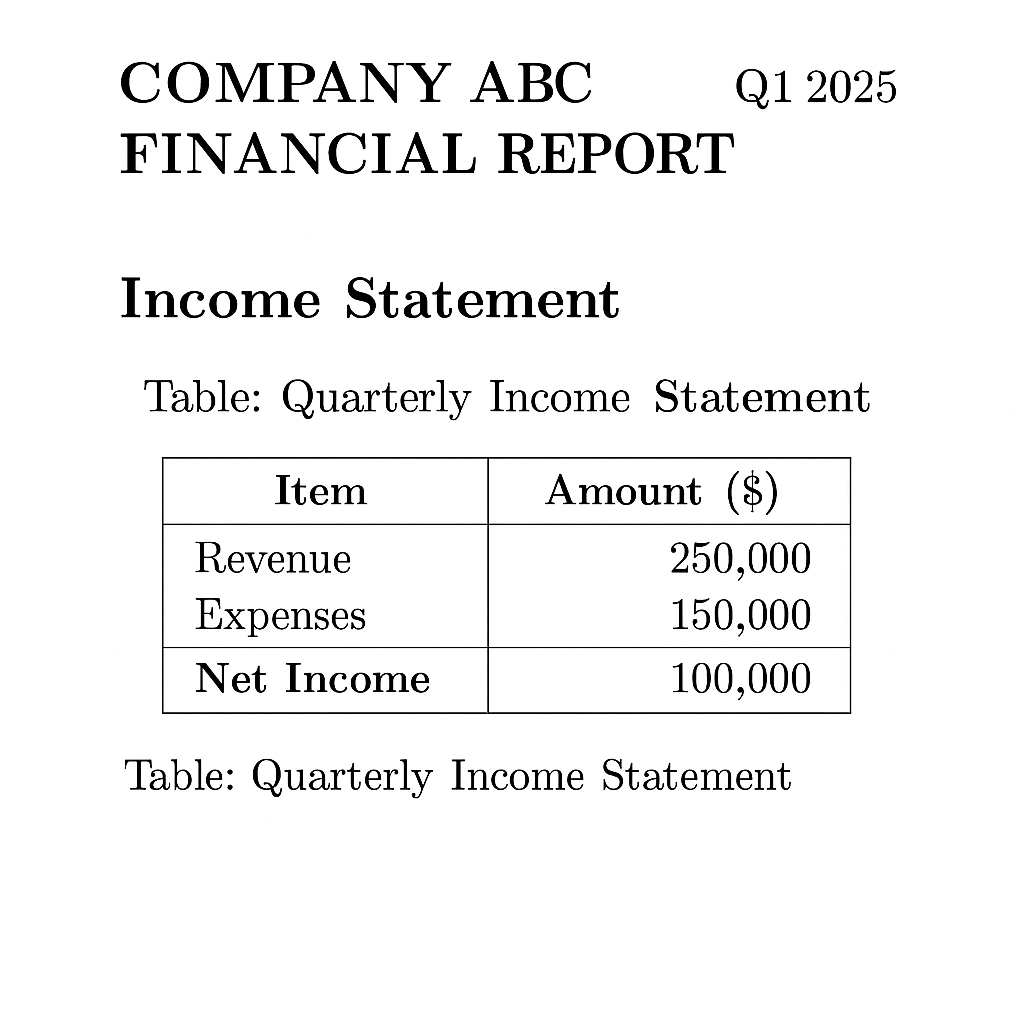
\includegraphics[width=0.85\textwidth]{figs/financial_report.png}
  \caption{Ảnh minh họa tệp báo cáo tài chính gốc được dùng trong thực nghiệm}
\end{figure}
\section{Biểu diễn thuật toán}

Hình ảnh sau đây biểu diễn trực quan thuật toán kiểm tra số nguyên tố đã được áp dụng trong quá trình xử lý báo cáo.

\begin{figure}[H]
    \centering
    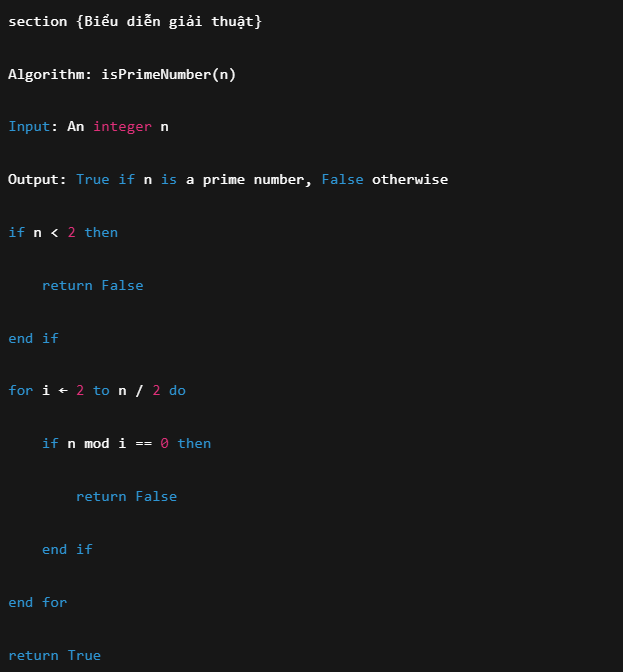
\includegraphics[width=0.75\textwidth]{figs/LyX.PNG}
    \caption{Biểu diễn thuật toán kiểm tra số nguyên tố bằng LyX}
\end{figure}

\section{Phân tích kết quả thực nghiệm}

Dưới đây là biểu đồ phân tích kết quả thực nghiệm, thể hiện hiệu suất và thời gian xử lý của quá trình nén, mã hóa và truyền dữ liệu trong các điều kiện khác nhau.

\begin{figure}[H]
    \centering
    \includegraphics[width=0.85\textwidth]{figs/ICC_plots.pdf}
    \caption{Biểu đồ phân tích hiệu suất xử lý và truyền báo cáo}
\end{figure}


---

